\documentclass[11pt]{article}
\usepackage{MyTemplate}
\begin{document}
\thispagestyle{empty}
\settextfont[Scale=1.2]{B Nazanin}
\begin{center}

\includegraphics{logo}
\vskip 1cm
{\bf
دانشگاه صنعتی شریف\\ دانشکده مهندسی کامپیوتر\\ سمینار کارشناسی ارشد گرایش هوش مصنوعی\\
\vskip 1cm
عنوان:\\
دسته‌بندی ریزدانه‌ای  تصاویر‬\\
\lr{‫Fine-grained Image Classification}
\vskip 1cm
نگارش:\\
یاسر سوری\\
۹۲۲۰۴۷۴۴\\
\vskip 1cm
استاد راهنما:\\
دکتر شهره کسایی\\
\vskip 1cm
استاد ممتحن داخلی:\\
دکتر محمد تقی منظوری شلمانی\\

\vskip 3.5cm

}
شهریور ۹۳
\newpage
\end{center}



\usepackage{pifont}
\newcommand{\cmark}{\ding{51}}

\settextfont[Scale=1]{XB Yas}
\setlatintextfont[Scale=0.95]{Times New Roman}
%\settextfont{B Nazanin}
%\settextfont{XB Yas}
%\settextfont{XB Kayhan}

{\bf {چکيده: }}
دسته‌بندی تصاویر ریزدانه‌ای عبارت است از دسته‌بندی تصاویر در حالتی که دسته‌های مورد نظر همگی زیر دسته‌ی یک دسته‌ی کلی‌تر هستند. برای مثال برای زیر دسته‌ی کلی پرندگان ما می‌توانیم گونه‌های مختلف پرندگان را در نظر بگیریم. در این حالت خاص مسئله دسته‌ها معمولاً از نظر ظاهری بسیار به یکدیگر شبیه هستند به گونه‌ای که افراد غیر متخصص نمی‌توانند دسته‌ها را از یکدیگر تمایز دهند. در چنین شرایطی راه حل‌های ارائه شده برای مسئله دسته‌بندی تصاویر معمولی اکثراً نتایج خوبی کسب نمی‌کنند. لذا ارائه روش‌هایی جدید برای حل این مسئله لازم است.
در این گزارش ابتدا به مرور روش‌های مهم در دسته‌بندی تصاویر معمولی و سپس به مرور روش‌های ارائه شده برای دسته‌بندی تصاویر ریزدانه‌ای می‌پردازیم. سپس روش انتخاب شده و دلایل انتخاب آن را بررسی می‌کنیم.
% تعریف مختصر راه حل
% در این گزارش چه مواردی بیان خواهد شد و چه نتیجه‌ای گرفته خواهد شد.


{\bf  { واژه‌های کلیدی: }}
بینایی کامپیوتری، بازشناسی شیء، دسته‌بندی تصاویر، بازشناسی ریزدانه‌ای، دسته‌بندی تصاویر ریزدانه‌ای.

\setlength{\parindent}{0.25in} %The indent of the paragraph first line

%%%%%%%%%%%%%%%%%%%%%%%%%%%%%%%%%%%%%%%%%%%%%%%%%%%%%%%%%%%%%%%%%
\section{مقدمه}\label{sec:intro}
% تعریف مسئله
در دسته‌بندی تصویر 
\footnote{\lr{Image classification}}
هر تصویر با توجه به محتوایش دسته‌بندی می‌شود. برای مثال آیا تصویر شامل شی‌ء خودرو هست یا خیر. معمولاً در بینایی کامپیوتری مسئله بدین صورت است که تعدادی دسته‌ی مشخص را در نظر می‌گیریم (مثلاً انسان، خودرو، ساختمان، تلویزیون، صندلی، اسب و ...) سپس طبق چارچوب معمول یادگیری ماشین، توسط تعدادی تصویر شامل یکی از دسته‌ها (نمونه‌های مثبت) و تعدادی تصویر بدون شی‌ای از آن دسته (نمونه‌های منفی) یادگیری برای آن دسته انجام می‌شود. در نهایت پس از یادگیری تمام دسته‌ها در مواجهه با تصویر جدید لازم است تشخیص دهیم که آیا شی‌ای از هر کدام از آن دسته‌های مورد بررسی در تصویر وجود دارد یا خیر.
برای نمونه به شکل
\ref{fig:intro:img_class_data}
توجه کنید. در این شکل داده‌های آموزشی و آزمایشی برای دسته‌بند دسته‌ی «صفحه کلید
\footnote{\lr{Computer - Keyboard}}
» از پایگاه داده
\lr{Caltech256} \cite{caltech256}
 نشان داده شده است.

\begin{figure}[b!]
	\centering
	\begin{subfigure}[h]{0.5\textwidth}
		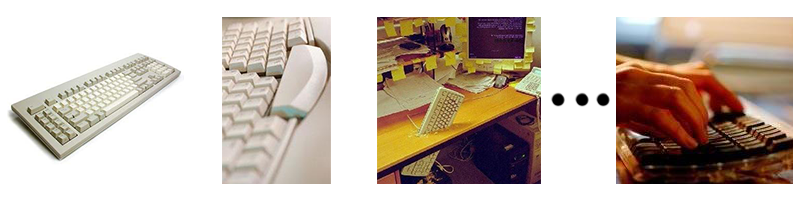
\includegraphics[width=\textwidth]{keyboard_positive}
		\caption{نمونه‌های مثبت، شامل شی‌ء صفحه کلید}
		\label{fig:intro:img_class_data:train_pos}
	\end{subfigure}
	\begin{subfigure}[h]{0.5\textwidth}
		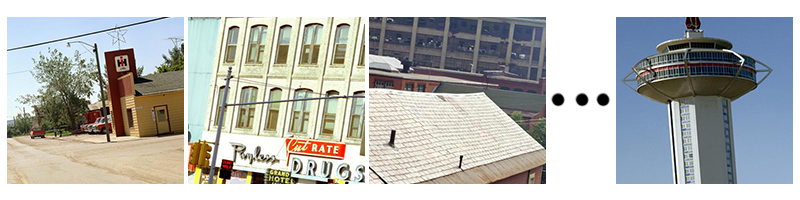
\includegraphics[width=\textwidth]{keyboard_negative}
		\caption{نمونه‌های منفی، بدون شی‌ء صفحه کلید}
		\label{fig:intro:img_class_data:train_neg}
	\end{subfigure}
	\begin{subfigure}[h]{0.5\textwidth}
		\centering
		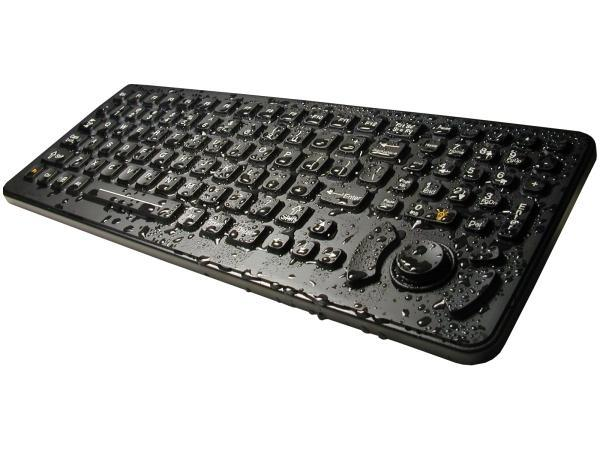
\includegraphics[width=0.5\textwidth]{keyboard_q}
		\caption{تصویر جدید آزمایشی}
		\label{fig:intro:img_class_data:query}
	\end{subfigure}
 
	\caption{‌نمونه‌ای از تصاویر آموزشی و آزمایشی سامانه دسته‌بند تصاویر برای دسته‌ی «صفحه کلید». انتخاب شده از پایگاه داده‌ی
\lr{Caltech256} \cite{caltech256}.
			سامانه لازم است با مشاهده نمونه‌های مثبت \ref{fig:intro:img_class_data:train_pos} و نمونه‌های منفی \ref{fig:intro:img_class_data:train_neg} یادگیری را انجام داده و بتواند پاسخ دهد که در تصویر جدید آزمایشی \ref{fig:intro:img_class_data:query} آیا صفحه کلید وجود دارد یا خیر. برای این نمونه پاسخ مثبت است.
			}
	\label{fig:intro:img_class_data}
\end{figure}
چالش‌های اصلی این مسئله تنوع زیاد اشیاء درون هر کدام از دسته‌ها، نحوه‌ی عکس برداری و وجود اشیاء دیگر در تصویر است که باعث ایجاد تصاویری با تنوع بالا می‌شود. مدل کردن این تنوع مربوط به اشیاء هر دسته باید همزمان با توانایی تمایز بین دسته‌های مختلف باشد. برای نمونه شکل
\ref{fig:intro:img_class_discrim}
تصویری از دو دسته مختلف مربوط به پایگاه داده
Imagenet \cite{imagenet}
را نمایش می‌دهد. مدل دسته‌بند باید توانایی تمایز بین این دو دسته شبیه به هم را داشته باشد.

\begin{figure}[t]
	\centering
	\begin{subfigure}[h]{0.35\textwidth}
		\centering
		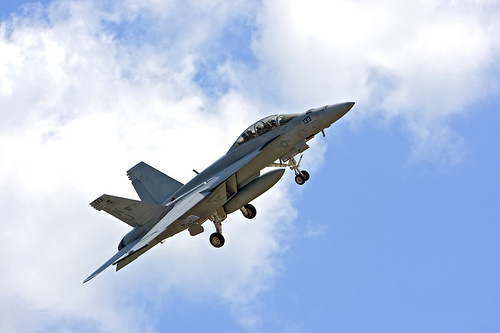
\includegraphics[height=4 cm]{fighter}
		\caption{هواپیمای جنگنده}
	\end{subfigure}
	\begin{subfigure}[h]{0.35\textwidth}
		\centering
		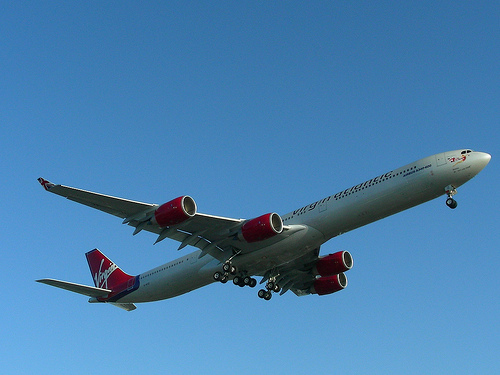
\includegraphics[height=4 cm]{airliner}
		\caption{هواپیمای مسافربری}
	\end{subfigure}
	\caption{نمونه‌ای از دو دسته‌ی متفاوت ولی شبیه به هم از پایگاه داده
Imagenet \cite{imagenet}.
مدل دسته‌بند علاوه بر توانایی مدل‌سازی تفاوت‌های داخل دسته‌ای، باید توانایی تمایز بین دسته‌های گاها شبیه به یکدیگر را داشته باشد.
}
	\label{fig:intro:img_class_discrim}
\end{figure}

اگر در دسته‌بندی تصویر، دسته‌های مورد بررسی زیر دسته‌ی
\footnote{\lr{Subclass}}
یک دسته‌ی کلی‌تر باشند(مانند گونه‌های مختلف پرندگان، مدل‌های مختلف خودروهای سواری و انواع مختلف هواپیماها)، آنگاه مسئله را «دسته‌بندی ریزدانه‌ای تصویر
\footnote{\lr{Fine-grained image classification}}»
می‌نامند. در دسته‌بندی ریزدانه‌ای تصویر معمولاً شباهت دسته‌ها به یکدیگر بسیار زیاد است به نحوی که افراد غیر متخصص نمی‌توانند به راحتی این دسته‌ها را بازشناسی نمایند. برای نمونه در شکل
\ref{fig:intro:terns}
چند گونه‌ی مختلف از پرستوی دریایی
\footnote{\lr{Tern}}
متعلق به پایگاه داده
\lr{CUB-200-2011} \cite{cub2002011}
نمایش داده شده است. همانگونه که می‌بینید با اینکه این نمونه‌ها به نحوی انتخاب شده‌اند که وضعیت مشابهی دارند، هنوز هم پیدا کردن ویژگی‌های تمایز دهنده بین گونه‌های مختلف کار بسیار سختی است و نیاز به تخصص دارد.

\begin{figure}[h]
	\centering
	\begin{subfigure}[h]{0.23\textwidth}
		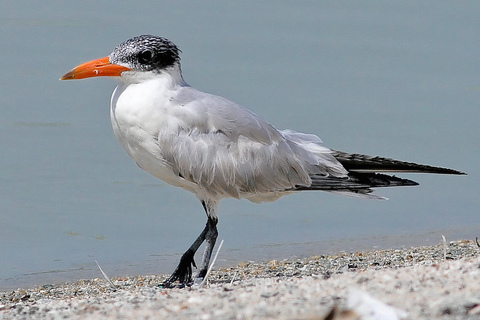
\includegraphics[height=2.5 cm]{Caspian_Tern}
		\caption{\lr{The Caspian tern}}
		\label{fig:intro:terns:1}
	\end{subfigure} 
	\begin{subfigure}[h]{0.23\textwidth}
		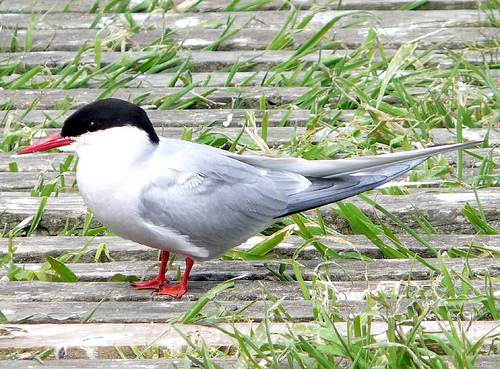
\includegraphics[height=2.5 cm]{Artic_Tern}
		\caption{\lr{The Artic tern}}
		\label{fig:intro:terns:2}
	\end{subfigure}
	\begin{subfigure}[h]{0.23\textwidth}
		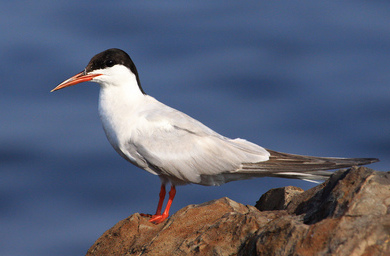
\includegraphics[height=2.5 cm]{Common_Tern}
		\caption{\lr{The common tern}}
		\label{fig:intro:terns:3}
	\end{subfigure}
	\begin{subfigure}[h]{0.23\textwidth}
		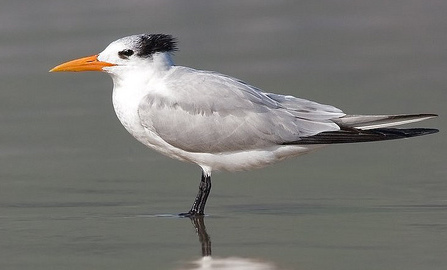
\includegraphics[height=2.5 cm]{Elegant_Tern}
		\caption{\lr{The elegent tern}}
		\label{fig:intro:terns:4}
	\end{subfigure}
	\caption{چهار گونه‌ی مختلف از پرستوهای دریایی متعلق به پایگاه داده
\lr{CUB-200-2011} \cite{cub2002011}.
شباهت بسیار زیاد بین دسته‌های مختلف کار را حتی برای افراد عادی (غیر متخصص) بسیار سخت می‌کند.
}
	\label{fig:intro:terns}
\end{figure}

روش‌های دسته‌بندی تصویر معمولی در مسايل دسته‌بندی ریزدانه‌ای اکثراً موفق نیستند. دلیل اصلی این عدم موفقیت وجود ویژگی‌های بسیار اندک و شدیداً محلی تمایزدهنده
\footnote{\lr{Discriminative}}
برای دسته‌های ریزدانه ایست. برای مثال دو گونه‌ی
\lr{elegent tern} در شکل \ref{fig:intro:terns:4}
و
\lr{common tern} در شکل \ref{fig:intro:terns:3}
فقط در رنگ پا و شکل تاج با یکدیگر تفاوت دارند و در سایر اجزا غیر قابل تمایز هستند. 

% کاربردها
مسئله دسته‌بندی تصویر را می‌توان به دلیل کاربردهای زیاد آن یکی از اساسی‌ترین مسائل بینایی کامپیوتری دانست که امروزه مورد علاقه محققین در سطح جهان است. نتایج بهترین روش‌های دسته‌بندی تصاویر بر روی بزرگ‌ترین پایگاه داده‌های دسته‌بندی تصویر نشان داده است که اکثر خطای این روش‌ها مربوط به دسته‌هایی است که از نظر ظاهری به یکدیگر بسیار نزدیک هستند. به عبارت دیگر خطای این روش‌ها اکثراً خطای ریزدانه ایست (به بخش
\ref{sec:img_class:conclusion}
مراجعه شود). لذا برای تقویت روش‌های دسته‌بندی تصویر، تمرکز بر روی دسته‌بندی ریزدانه‌ای اهمیت زیادی دارد.
از جمله کاربردهای مسئله دسته‌بندی ریزدانه‌ای تصویر می‌توان به موتورهای جستجو و بازیابی محتوا محور تصاویر
\footnote{\lr{Content based image retrieval}}
(برای مثال پیدا کردن مدل خاصی از یک خودرو در بین انبوهی از تصاویر)، سامانه‌های کمک آموزشی (آموزش گونه‌های مختلف حیوانات) و سامانه‌های نظارتی
\footnote{\lr{Surveillance systems}}
(کنترل ترافیک و تشخیص مدل‌های مختلف خودرو) اشاره کرد.

%آنچه خواهید خواند
در ادامه ابتدا در بخش
\ref{sec:img_class}
به معرفی سامانه‌های دسته‌بند تصویر معمولی و کارهای پیشین در این زمینه خواهیم پرداخت. سپس در بخش
\ref{sec:fg_class}
به معرفی روش‌های دسته‌بندی ریزدانه‌ای تصاویر و پایگاه داده‌های مرتبط با آن خواهیم پرداخت. در انتها در بخش
\ref{sec:conc}
چند آزمایش و ایده برای ادامه کار به همراه نتیجه‌گیری‌ها و جمع‌بندی را مطرح می‌کنیم.

%%%%%%%%%%%%%%%%%%%%%%%%%%%%%%%%%%%%%%%%%%%%%%%%%%%%%%%%%%%%%%%%%
\section{دسته‌بندی تصاویر معمولی}\label{sec:img_class}
در این گزارش دسته‌بندی غیر ریزدانه‌ای تصاویر را معمولی خطاب می‌کنیم. همانطور که در مقدمه (بخش
\ref{sec:intro})
بیان شد، در دسته‌بندی تصویر، باید تصویر را با توجه به محتوایش دسته‌بندی کنیم. برای این منظور دسته‌ها را می‌توان به چندین صورت تعریف کرد. دسته‌های به صورت سنتی به دو دسته تقسیم می‌شدند: دسته‌بندی شیء
\footnote{\lr{Object classification}}
(برای مثال
\lr{Caltech101/256} \cite{caltech101, caltech256}
و
\lr{PASCAL VOC} \cite{pascalvoc})
و دسته‌بندی صحنه
\footnote{\lr{Scene classification}}
(برای مثال
\lr{MIT 67 Scene} \cite{mit67scene}).
در دسته‌بندی شیء لازم است که وجود و یا عدم وجود شی‌ای از دسته‌های مورد نظر در تصویر را تشخیص دهیم و لازم نیست که مکان آن شی‌ء را در تصویر مشخص نماییم. در دسته‌بندی صحنه لازم است از بین صحنه‌های مورد بررسی تشخیص دهیم که تصویر متعلق به کدام صحنه است. برای مثال تصویر
\ref{fig:img_class:object_vs_scene}
را در نظر بگیرید. فرض کنید که شی‌ء‌های هواپیما، اتوبوس، خودرو سواری و اسب را در مد نظر داریم و می‌خواهیم دسته‌بندی شی‌ء را برای تصویر
\ref{fig:img_class:object_vs_scene}
انجام دهیم. در این حالت خروجی سامانه باید بدین صورت باشد: «هواپیما در تصویر وجود دارد. اوتوبوس در تصویر وجود دارد. خودرو سواری و اسب در تصویر وجود ندارد». حالا اگر صحنه‌های فرودگاه، فروشگاه و مسجد را در نظر بگیریم و بخواهیم دسته‌بندی صحنه را برای تصویر انجام دهیم، خروجی سامانه باید بدین صورت باشد: «تصویر صحنه فرودگاه را نشان می‌دهد».
\begin{figure}[t!]
	\centering
	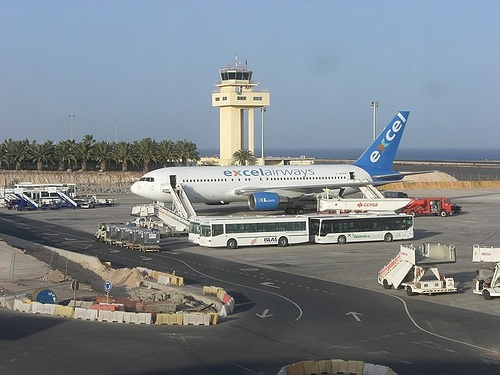
\includegraphics[height=4 cm]{object_vs_scene}
	\caption{نمونه خروجی سامانه‌های دسته‌بندی شی‌ء و صحنه. برای دسته‌بندی شی‌ء اگر شی‌ءهای هواپیما، اتوبوس، خودرو سواری و اسب را مد نظر داشته باشیم، خروجی سامانه باید بدین صورت باشد: «هواپیما در تصویر وجود دارد. اوتوبوس در تصویر وجود دارد. خودرو سواری و اسب در تصویر وجود ندارد».
برای دسته‌بندی صحنه اگر صحنه‌های فرودگاه، فروشگاه و مسجد را در نظر بگیریم، خروجی سامانه باید بدین صورت باشد: «تصویر صحنه فرودگاه را نشان می‌دهد».}
	\label{fig:img_class:object_vs_scene}
\end{figure}

در سال‌های اخیر محققین به دسته‌بندی‌های دیگری نیز روی آورده‌اند. برای نمونه می‌توان به بازشناسی صفت
\footnote{\lr{Attribute recognition}}\cite{farhadi2009}
و بازشناسی افعال
\footnote{\lr{Action recognition}}
در تصاویر
\cite{bangpeng2011}
اشاره کرد.
در این گزارش تمرکز بر دسته‌بندی شی‌ء خواهد بود. در ادامه برخی روش‌های دسته‌بندی شیء در تصاویر را بررسی خواهیم کرد.

\subsection{روش‌های مبتنی بر لغت‌نامه}\label{sec:img_class:vocab_based}
روش‌های مبتنی بر لغت‌نامه از قدیمی‌ترین روش‌ها در دسته‌بندی تصویر هستند که هنوز هم مورد استفاده قرار می‌گیرند. ایده اولیه این روش‌ها از تحقیقات پردازش متن گرفته شده است. در پردازش متن، یک لغت‌نامه داریم و یک متن  و می‌خواهیم متن را دسته‌بندی کنیم. اگر فرکانس لغات داخل متن را محاسبه کنیم، می‌بینیم که لغات پر تکرار در متون یک دسته‌ی خاص مشترک هستند. این مشاهده باعث شد که روش‌های مبتنی بر لغت‌نامه برای دسته‌بندی متن مورد استفاده قرار بگیرند.

محققان بررسی کردند که همین مشاهدات در مورد تصاویر نیز برقرار است. برای مثال فرض کنیم که لغات را در تصاویر به صورت تکه‌ای از تصویر تعریف کنیم. حال اگر لغت معادل دهان، چشم و بینی را در تصویری مشاهده کنیم می‌توانیم نتیجه بگیریم که به احتمال زیاد تصویر مربوط به یک چهره است. البته مسئله برای تصویر از متن پیچیده‌تر است، زیرا لغت‌نامه‌ای در دسترس نیست و همچنین پیدا کردن لغت‌ها کار مشکلی است.

کلیت این روش‌ها بر پایه‌ی دسته‌بندی در یادگیری ماشین است. بدین صورت که تعدادی تصویر آموزشی و دسته‌های آن‌ها (برچسب) را در اختیار داریم. ابتدا یک مدل دسته‌بند مثل
\lr{SVM} \cite{svm}
را انتخاب می‌کنیم و با داده‌های آموزشی مدل را آموزش می‌دهیم. حال برای داده‌های آزمایشی با استفاده از مدل برچسب را تخمین می‌زنیم. برای استفاده از این چارچوب دسته‌بندی باید نمایش برداری مناسبی از تصاویر داشته باشیم که در آموزش و آزمایش طول یکسانی داشته باشد. این نمایش برداری توسط مرحله‌ی کدینگ
\footnote{\lr{Coding}}
همانطور که در شکل
\ref{fig:img_class:pipe}
نشان داده شده است، بدست می‌آید.
در ادامه به راه حل‌های مختلف برای ساخت لغت‌نامه و کدینگ می‌پردازیم.
\subsubsection{ساخت لغت‌نامه}\label{sec:img_class:vocab}
در روش‌های مبتنی بر لغت‌نامه، ساخت لغت‌نامه یکی از اساسی‌ترین گام‌هاست و از آنجایی که فقط کافی است یک بار ساخته شود و در طول اجرای برنامه نیاز به بازسازی ندارد اگر زمان زیادی هم صرف این کار شود ایرادی ندارد.
\begin{figure}[t!]
	\centering
	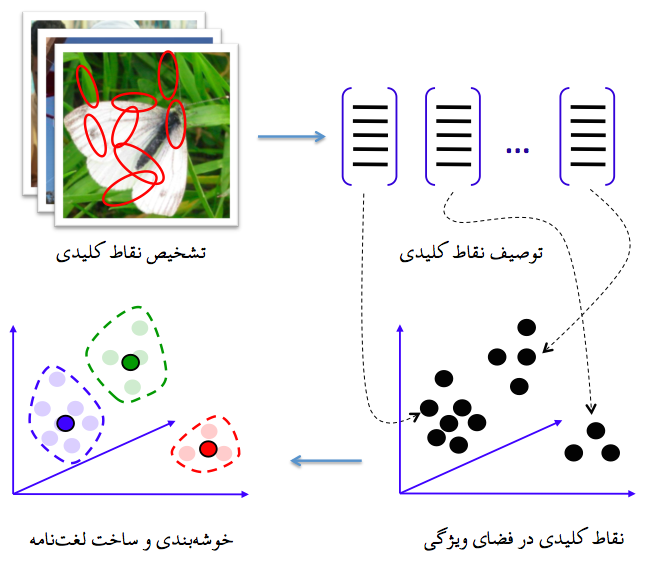
\includegraphics[height= 7 cm]{bow_vocab}
	\caption{ساخت لغت‌نامه در روش کیسه‌ای از لغات}
	\label{fig:img_class:bow_vocab}
\end{figure}
در شکل
\ref{fig:img_class:bow_vocab}
یکی از ابتدایی‌ترین و پر کاربردترین روش‌های ساخت لغت‌نامه را مشاهده می‌کنید
\cite{csurka2004}.
گام‌های این روش برای ساخت لغت‌نامه بدین صورت است:
\begin{itemize}
	\item در مجموعه تصاویر آموزشی نقاط کلیدی
	\footnote{\lr{Keypoints}}
	را توسط الگوریتمی مثل
	\lr{Harris-Affine} \cite{harris_affine}
	یا به صورت چگال
	\footnote{Dense}
	تشخیص می‌دهیم.

	\item نقاط کلیدی را توسط توصیفگری مثل
	\lr{SIFT} \cite{sift}
	توصیف می‌کنیم.
	\item با اعمال یکی از روش‌های تدریج برداری
	\footnote{\lr{Vector quantization}}
	مثل
	\lr{KMeans}
	توصیفگر هر قطعه از تصاویر را به یکی از مراکز خوشه‌های
	\footnote{\lr{Clusters}}
	لغت‌نامه اختصاص می‌دهیم.
\end{itemize}
مراکز خوشه‌ها همان لغت‌نامه خواهند بود. این روش یکی قدیمی‌ترین روش‌های ساخت لغت‌نامه است. بعدها روش‌های پیچیده‌تری مثل
\cite{adapted_vocab, jurie2005}
برای این کار معرفی شدند. 
\subsubsection{روش کیسه‌ای از لغات}
روش «کیسه‌ای از لغات»
\footnote{\lr{Bag of keypoints}}
از قدیمی‌ترین روش‌ها برای مسئله دسته‌بندی است
\cite{csurka2004}.
در این روش «کیسه‌ای از لغات» به هیستوگرام تعداد تکرارهای لغات درون لغت‌نامه در تصویر گفته می‌شود. لغت‌نامه همانطور که در قسمت
\ref{sec:img_class:vocab}
بیان شد ساخته می‌شود. شمای کلی این روش را می‌توان در تصویر
\ref{fig:img_class:pipe:bow}
مشاهده کرد.

\begin{figure}[t]
	\centering
	\begin{subfigure}[h]{0.7\textwidth}
		\centering
		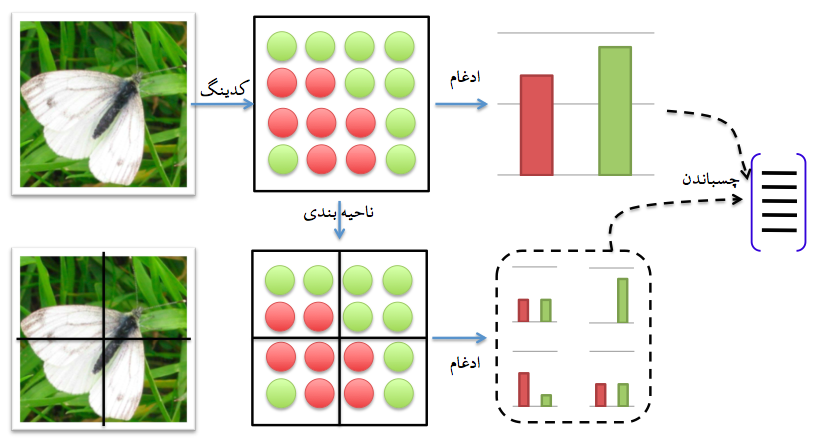
\includegraphics[height=5 cm]{spm}
		\caption{روش تطبیق هرم مکانی}
		\label{fig:img_class:pipe:spm}
	\end{subfigure}
	\begin{subfigure}[h]{0.3\textwidth}
		\centering
		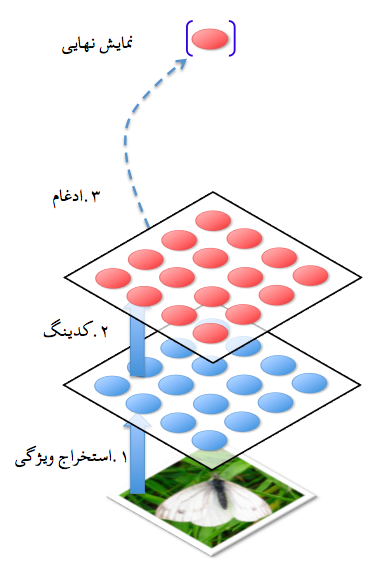
\includegraphics[height=7 cm]{img_class_pipe_bow}
		\caption{روش کیسه‌ای از لغات}
		\label{fig:img_class:pipe:bow}
	\end{subfigure}
	\begin{subfigure}[h]{0.3\textwidth}
		\centering
		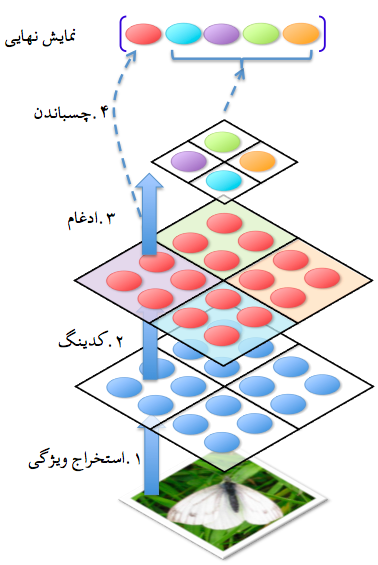
\includegraphics[height=7 cm]{img_class_pipe_spm}
		\caption{روش‌های برپایه‌ی تطبیق هرم مکانی}
		\label{fig:img_class:pipe:gen}
	\end{subfigure}
	\caption{نمای کلی روش‌های برپایه لغت‌نامه}
	\label{fig:img_class:pipe}
\end{figure}
ابتدا در گام استخراج ویژگی، از تصویر ورودی نقاط کلیدی را استخراج و توصیف می‌کنیم، این توصیف‌ها توسط دایره‌های آبی رنگ نشان داده شده‌اند. سپس در گام کدینگ این توصیف‌ها را به نزدیک‌ترین لغت درون لغت‌نامه نگاشت می‌کنیم که حاصل کدها (دایره‌های قرمز) خواهند بود. نهایتاً در مرحله‌ی ادغام
\footnote{\lr{Pooling}}
تمام کدها را توسط میانگین گیری به نمایش نهایی تبدیل می‌کنیم. این ادغام را «ادغام میانگین
\footnote{\lr{Average pooling}}» می‌نامند.

به صورت ریاضی این روش را می‌توان بدین صورت مطرح کرد. فرض کنید که $X$ مجموعه‌ی توصیف‌های نقاط کلیدی استخراج شده از تصویر باشد، یعنی:
$X = [x_1, x_2, ..., x_N] \in \mathbb{R}^{D \times N}$.
با فرض داشتن لغت‌نامه‌ای با $M$ لغت،
$B = [b_1, b_2, ..., b_M] \in \mathbb{R}^{D \times M}$
حال باید $x_i$ها را به برداری $M$ بعدی تبدیل کنیم. سپس از این بردارهای $M$ بعدی می‌توان نمایش نهایی را ساخت.
در روش کیسه‌ای از لغات از تدریج برداری استفاده می‌شود که مسئله بهینه‌سازی زیر را حل می‌کند.
\begin{equation}
	\begin{aligned}
		&\operatorname*{arg\,min}_C \sum_{i=1}^{N} || x_i - B c_i ||^2 \\
		&{\,\,\,\,} \textit{s.t.} || c_i ||_{\ell^0} = 1, || c_i ||_{\ell^1} = 1, c_i \succeq 0, \forall i
	\end{aligned}
\label{equ:img_class:vq}
\end{equation}

با فرض اینکه کدینگ
$C = [c_1, c_2, ..., c_N] \in \mathbb{R}^{M \times N}$
مجموعه کد‌های مربوط به $X$ هستند.
شرط
$|| c_i ||_{\ell^0} = 1$
(نرم صفرم $c_i$ها) در بهینه‌سازی
\ref{equ:img_class:vq}
بدین معناست که فقط یک عنصر غیر صفر در $c_i$ وجود داشته باشد. همچنین شروط
$|| c_i ||_{\ell^1} = 1, c_i \succeq 0$
بدین معناست که آن عنصر غیر صفر باید برابر با مثبت یک باشد. در عمل این مسئله بهینه‌سازی همانطور که گفته شد با جستجوی نزدیک‌ترین همسایه در فضای توصیف حل می‌شود.

این روش ساده در پایگاه داده‌های ابتدایی نتایج قابل قبولی داشت. مهم‌ترین نکته قوت این روش مقاوم بودن در مقابل تبدیل‌های انتقالی است. بدین معنا که برای این روش فرقی نمی‌کند که شی‌ء در کدام قسمت تصویر وجود داشته باشد. از طرفی همین موضوع می‌توان باعث نقطه ضعف این روش شود، زیرا این نکته باعث می‌شود موقعیت مکانی ویژگی‌ها را حفظ نکند، که در نهایت باعث می‌شود توانایی مدل کردن شکل را نداشته باشد.

از بین توسعه‌هایی که به روش کیسه‌ای از لغت داده شد
\cite{jurie2005, nn_img_class, berg2005}
روش «تطبیق هرم مکانی
\footnote{\lr{Spatial pyramid matching}}» \cite{spm}
از دیگران نتایج بهتری داشت. در ادامه به بررسی این روش می‌پردازیم.
\subsubsection{روش تطبیق هرم مکانی}
این روش
\cite{spm}
سعی داشت که مشکل از دست دادن اطلاعات مکانی را در روش کیسه‌ای از لغات حل کند. کلیت این روش در شکل
\ref{fig:img_class:pipe:spm}
نشان داده شده است. در این روش تصویر به ناحیه‌های هرچه ریزتر تقسیم می‌شود و هیستوگرام کدها در هر کدام از زیر ناحیه‌ها محاسبه می‌شوند. و در انتها این هیستوگرام‌ها به عنوان نمایش نهایی کنار هم قرار داده می‌شود.

در این روش استخراج ویژگی و کدینگ دقیقاً مثل روش کیسه‌ای از لغات است. تنها تفاوت در گام ادغام رخ می‌دهد. (به شکل
\ref{fig:img_class:pipe:bow} و
\ref{fig:img_class:pipe:gen}
توجه نمایید)
در این گام ابتدا ناحیه‌بندی صورت می‌گیرید. زیر ناحیه‌های معمولاً به صورت
$2 ^ l \times 2 ^ l , l = 0, 1, 2$
هستند. در شکل
\ref{fig:img_class:pipe:spm}
زیر ناحیه‌های
$2 \times 2$ و $1 \times 1$
نشان داده شده است. سپس برای هر کدام از ناحیه‌های ادغام میانگین انجام می‌گیرد و هیستوگرام‌هایی تولید می‌شود. در نهایت گام چسباندن این هیستوگرام‌ها را کنار هم قرار داده و به نمایش نهایی تبدیل می‌کند.

یکی از نقطه ضعف‌های این روش این است که برای کسب نتایج خوب باید از دسته‌بندهای غیر خطی مثل
\lr{SVM}
با هسته‌های غیر خطی مثل
\lr{Chi-square} استفاده شود.
این موضوع باعث می‌شود که هزینه‌ی محاسباتی در گام آموزش
\BigO{n^3}
و در هنگام آزمایش
\BigO{n}
باشد که $n$ تعداد بردارهای پشتیبان
\footnote{\lr{Support Vector}}
است. دیگر نقطه ضعف مهم این روش که آن را از روش‌های کیسه‌ای از لغات به ارث برده است، خطای تدریج در مرحله‌ی کدینگ است. این خطا همانطور که در
\cite{nn_img_class}
به تفصیل به آن پرداخته شده است، مهم‌ترین نقطه ضعف این روش است.
برای بهبود مقیاس‌پذیری و از بین بردن خطای تدریج این روش محققان بر روی روش‌های کدینگ غیر خطی کار کردند که با دسته‌بندهای خطی نیز خوب کار کنند. در ادامه به برخی از این روش‌ها خواهیم پرداخت.
\subsubsection{روش‌های کدینگ تنک}
برای از بین بردن خطای تدریج، شرط قوی
$|| c_i ||_{\ell^0} = 1$
در معادله‌ی
\ref{equ:img_class:vq}
را می‌توان با اضافه کردن جمله‌ی منظم‌سازی
\footnote{\lr{Regularization}}،
نرم کرد. در روش «کدینگ تنک در تطبیق هرم مکانی»
\cite{scspm}
مرحله‌ی کدینگ با همین ایده به صورت زیر در آورده شده است:
\begin{equation}
	\operatorname*{arg\,min}_C \sum_{i=1}^{N} || x_i - B c_i ||^2  + \lambda || c_i ||_{\ell ^ 1}
	\label{equ:img_class:sc}
\end{equation}
جمله‌ی مرتب‌سازی با نرم ۱ باعث تنک شدن $c_i$ها خواهد شد
\cite{sc}.
بدین ترتیب می‌توان خطای تدریج را به میزان قابل ملاحظه‌ای کاهش داد. آزمایشات نشان داد که این روش کدینگ با دسته‌بندخطی از روش تطبیق هرم مکانی بسیار بهتر عمل می‌کند
\cite{scspm}.
لازم به ذکر است که ساختار کلی این روش‌ها مانند شکل
\ref{fig:img_class:pipe:gen}
است و فقط در مرحله‌ی کدینگ با یکدیگر تفاوت دارند.

همچنین روش‌های دیگری مثل
\cite{llc, fisher_kernel, fisher_kernel_im}
برای کدینگ مطرح شدند که نتایج دسته‌بندی را بهبود می‌دادند، که بدلیل کمبود فضا از توضیح آن‌ها خودداری می‌کنیم. در
\cite{devil_coding}
مقایسه‌ی کاملی بین روش‌های کدینگ انجام شده است، در نهایت می‌توان گفت بهترین نتیجه برای دسته‌بندی توسط کدینگ هسته‌ی فیشر
\cite{fisher_kernel_im}
بدست می‌آید.
\subsection{روش‌های مبتنی بر یادگیری عمیق}\label{sec:img_class:dl}
روش‌های مبتی برا یادگیری عمیق
\footnote{\lr{Deep learning}}
از سال‌های قبل در بینایی کامپیوتری استفاده می‌شدند
\cite{lenet}.
اما تا سال ۲۰۱۲ موفقیت چندانی در دسته‌بندی تصاویر واقعی نداشتند. در سال ۲۰۱۲ در مقاله‌ی مهمی از دانشگاه تورنتو
\cite{alexnet}
شبکه‌ی عصبی عمیقی معرفی شد که توجه همه را به خود جمع کرد. این شبکه‌ی عصبی موسوم به
\lr{AlexNet}
در مسابقات دسته‌بندی تصویر معتبر
\lr{ILSVRC}\cite{ilsvrc}
در سال ۲۰۱۲ توانست با اختلاف قابل ملاحظه‌ی از نفر دوم، اول شود. از این به بعد بود که محققان و صنعتگران از تمام جهان متوجه روش‌های یادگیری عمیق و قابلیت‌های آن در عرصه‌های مختلف شدند.

کمی قبل‌تر از معرفی
\lr{AlexNet}
محققان متوجه رشد کم در بهبود روش‌های بازشناسی تصویر شده بودند و در پی این بودند که بدانند چرا انسان‌ها قدرت بسیار بالایی در بازشناسی تصویر دارند ولی هوش‌ مصنوعی هنوز در این زمینه ضعف زیادی دارد. تعدادی از محققین با انجام آزمایشات گسترده بر روی انسان و روش‌های یادگیری ماشین متوجه شدند
\cite{parikh2010}
که نقطه ضعف روش‌های بینایی ماشین در ویژگی‌هایی (ویژگی‌هایی مثل
\lr{SIFT} \cite{sift} و \lr{HOG} \cite{hog})
است که استفاده می‌کند. به عبارت دیگر توانایی بالای انسان نه به خاطر آموزش با داده‌های آموزشی بیشتر و نه به خاطر مدل دسته‌بندی پیشرفته‌تر، بلکه بیشتر به خاطر ویژگی‌های بهتری است که استفاده می‌کند.

یکی از محرک‌های اصلی روش‌های یادگیری عمیق همین مسئله بود، به عبارت دیگر این روش‌ها نه تنها دسته‌بند، بلکه خود ویژگی‌ها را نیز با داده‌های آموزشی یاد می‌گیرند.

\subsection{نتیجه‌گیری}\label{sec:img_class:conclusion}
\begin{figure}[t]
	\centering
	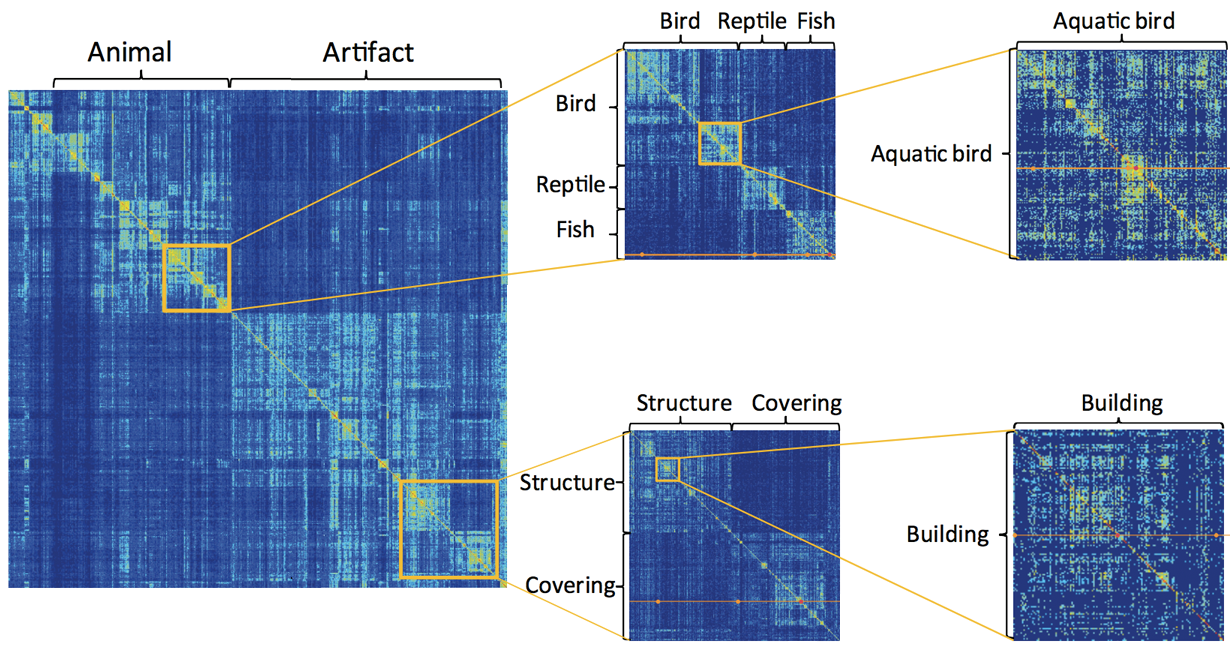
\includegraphics[height= 4 cm]{imagenet_conf}
	\caption{ماتریس ابهام برای پایگاه داده‌ی
	\lr{ImageNet} و ساختار درون آن}
	\label{fig:img_class:imagenet_conf}
\end{figure}
در این بخش مرور مختصری بر روش‌های پایه‌ای و مهم در دسته‌بندی تصویر داشتیم. در بین این روش‌ها آن‌هایی که برپایه‌ی لغت‌نامه هستند، بهترین نتیجه را با کدینگ هسته‌ی فیشر کسب می‌کنند. البته در مجموع روش‌های بر پایه‌ی یادگیری عمیق به خاطر ویژگی‌هایی که یاد می‌گیرند بهترین عملکرد را دارند. در ادامه دلیل اصلی ورود به دسته‌بندی ریزدانه‌ای تصویر را مطرح می‌کنیم.

یکی از بهترین و بزرگترین پایگاه داده‌ها برای مقایسه‌ی روش‌های دسته‌بندی تصویر پایگاه داده‌ی
\lr{ImageNet} \cite{imagenet} است.
بر روی این پایگاه داده و زیر مجموعه‌ی آن یعنی
\lr{ILSVRC} \cite{ilsvrc}
روش‌های یادگیری عمیق مثل
\cite{alexnet, overfeat, deconv}
بهترین نتایج را کسب کرده‌اند. از نتایج این روش‌ها می‌توان نکات جالبی را استخراج کرد. برای نمونه تصویر
\ref{fig:img_class:imagenet_conf}
ماتریس ابهام
\footnote{\lr{Confusion matrix}}
را برای روش
\cite{deng2010}
بر روی پایگاه داده
\lr{ImageNet}
نشان می‌دهد. نکته‌ای که باید به آن توجه شود ساختار موجود در ماتریس ابهام است. همانطور که در تصویر نیز مشخص است، مدل دسته‌بند بیشترین ابهام را در دسته‌هایی دارد که به یکدیگر از نظر ظاهری و معنایی نزدیک هستند. برای نمونه در بین پرنده‌ها ابهام زیاد وجود دارد و از پرنده‌ها در بین پرنده‌های آبی ابهام زیادتر است. به عبارت دیگر ابهام در بین دسته‌های ریزدانه‌ای است. این موضوع باعث می‌شود که نتیجه بگیریم برای افزایش دقت روش‌های دسته‌بندی تمرکز بر روی دسته‌های ریزدانه‌ای بسیار مهم است. در ادامه به بررسی پایگاه داده‌ها و برخی از این روش‌ها می‌پردازیم.

%%%%%%%%%%%%%%%%%%%%%%%%%%%%%%%%%%%%%%%%%%%%%%%%%%%%%%%%%%%%%%%%%
\section{دسته‌بندی ریزدانه‌ای تصویر}\label{sec:fg_class}
\begin{figure}[t!]
	\centering
	\begin{subfigure}[h]{0.5\textwidth}
		\centering
		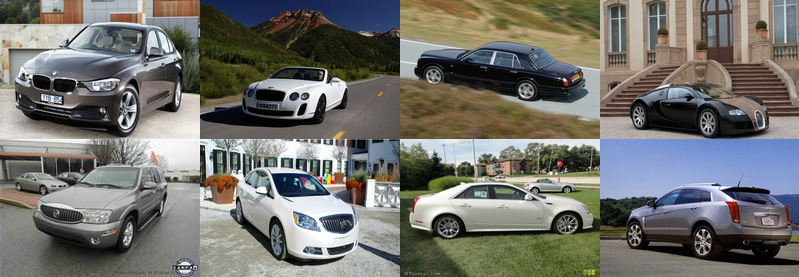
\includegraphics[width=\textwidth]{ds_cars}
		\caption{پایگاه داده‌ی ماشین‌های استنفورد}
		\label{fig:fg_class:ds:cars}
	\end{subfigure}
	\begin{subfigure}[h]{0.5\textwidth}
		\centering
		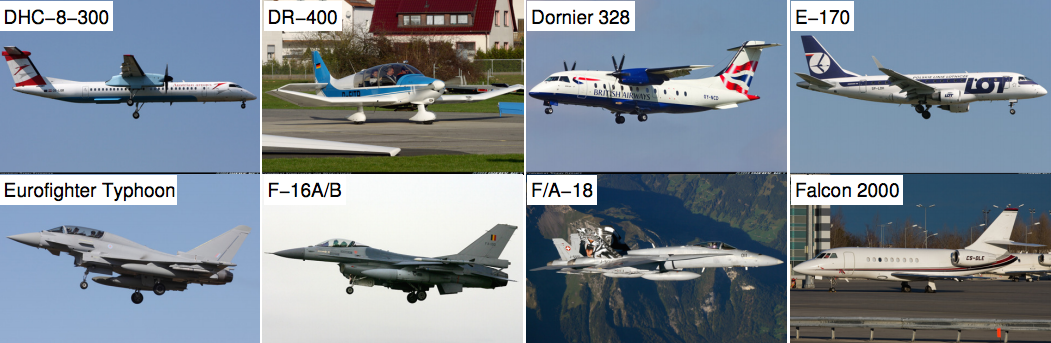
\includegraphics[width=\textwidth]{ds_aircraft}
		\caption{پایگاه داده‌ی هواپیماهای آکسفورد}
		\label{fig:fg_class:ds:aircraft}
	\end{subfigure}
	\begin{subfigure}[h]{0.5\textwidth}
		\centering
		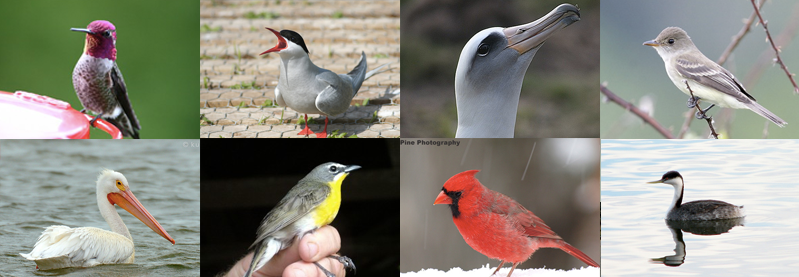
\includegraphics[width=\textwidth]{ds_birds}
		\caption{پایگاه داده‌ی پرندگان کلتک}
		\label{fig:fg_class:ds:birds}
	\end{subfigure}
	\caption{برخی از پایگاه داده‌های دسته‌بندی تصاویر ریزدانه‌ای}
	\label{fig:fg_class:ds}
\end{figure}
همانطور که گفته شد، اگر در دسته‌بندی تصویر، دسته‌های مورد بررسی زیر دسته‌ی
\footnote{\lr{Subclass}}
یک دسته‌ی کلی‌تر باشند(مانند گونه‌های مختلف پرندگان، مدل‌های مختلف خودروهای سواری و انواع مختلف هواپیماها)، آنگاه مسئله را «دسته‌بندی ریزدانه‌ای تصویر»
می‌نامند. در قسمت
\ref{sec:img_class:conclusion}
دلیل اصلی برای مطالعه بر روی دسته‌بندی ریزدانه‌ای را بررسی کردیم.

محققان در حوزه‌ی روانشناسی از سال‌ها قبل بر روی توانایی‌های انسان در دسته‌بندی مطالعه می‌کرده‌اند. برای نمونه دانشمندان نشان دادند
\cite{johnson1998}
که توانایی انسان برای انجام دسته‌بندی سطح اصلی
\footnote{\lr{Basic level}}
یا معمولی (تشخیص خودروی سواری از گربه یا تشخیص خیابان از خانه) خیلی قبل‌تر از توانایی انسان برای دسته‌بندی سطح فرعی
\footnote{\lr{Sub-ordinate level}}
یا ریزدانه‌ای توسعه می‌یابد. خیلی جالب است که در زمینه‌ی بینایی کامپیوتری هم همین منوال حفظ شده است، یعنی محققین ابتدا بر روی روش‌های دسته‌بندی سطح اصلی یا معمولی کار زیادی انجام داده‌اند و پیشرفت‌های خوبی حاصل شده است، امام اخیراً کار بر روی دسته‌بندی ریزدانه‌ای آغاز شده است. در ادامه به بررسی برخی از پایگاه داده‌های دسته‌بندی ریزدانه‌ای خواهیم پرداخت.

\subsection{پایکاه داده‌های دسته‌بندی ریزدانه‌ای}\label{sec:fg_class:datasets}
از بین پایگاه داده‌های مربوط به دسته‌بندی ریزدانه‌ای سه پایگاه داده مهم را انتخاب کرده‌ایم و مطالعات را بر روی آن‌ها انجام خواهیم داد. در ادامه ابعاد و نوع داده های موجود در این پایگاه داده‌ها را بررسی خواهیم کرد.
\subsubsection{ماشین‌های استنفورد}
این پایگاه داده در سال ۲۰۱۳ معرفی شد
\cite{stanford_cars}
و شامل ۱۶۱۸۵ تصویر از ۱۹۶ مدل مختلف خودروهای سواری است. برای هر خودرو جعبه‌ی دور
\footnote{\lr{Bounding box}}
خودرو هم داده شده است. که برای حذف پس زمینه کاربرد زیادی دارد. نمونه‌ای از تصاویر این پایگاه داده را در شکل
\ref{fig:fg_class:ds:cars}
مشاهده می‌کنید. برای این پایگاه داده چون می‌دانیم که خودروهای سواری را مطالعه می‌کنیم، بسیاری از روش‌ها
\cite{stanford_cars, krause2014, ramnath2014}
سعی می‌کنند که از دانش سه‌بعدی که در مورد خودروها داریم برای حل کردن بهتر مسئله استفاده کنند. این دانش سه‌بعدی شامل مدل سه‌بعدی و شکل خودروی سواری است که می‌توان از طریق اینترنت به آن‌ها دست پیدا کرد.

\subsubsection{هواپیماهای آکسفورد}
این پایگاه‌داده جدید در سال ۲۰۱۴ معرفی شد
\cite{oxford_aircraft}
و شامل ۷۵۰۰ تصویر از ۷۵ نوع مختلف هواپیما است. برای هر هواپیما جعبه دور هواپیما به همراه تعداد زیادی از ویژگی‌های اجزای آن (مثل تعداد موتور، تعداد چرخ، شکل بال‌ها و ...) به همراه ناحیه‌بندی
\footnote{\lr{Segmentation}}
آن جزء هواپیما موجود است. این پایگاه داده از نظر کامل بودن بسیار کامل است، ولی به خاطر جدید بودن هنوز مقاله‌ای به جز مقاله‌ی معرفی خود پایگاه داده از آن استفاده نکرده‌است. ضمناً اندازه داده‌های آن به نسبت دیگر پایگاه داده‌ها کم است. نمونه‌ای از تصاویر این پایگاه داده را در شکل
\ref{fig:fg_class:ds:aircraft}
مشاهده می‌کنید.

\subsubsection{پرندگان کلتک}
این پایگاه داده به نسبت قدیمی است و در سال ۲۰۱۰ و ۲۰۱۱ معرفی شده است
\cite{cub2002011, cub2002010}.
این پایگاه داده شامل ۱۱۷۸۸ تصویر از ۲۰۰ گونه مختلف از پرندگان است. برای هر پرنده ۱۵ جزء بدن (برای مثال بال راست، سر، پای چپ و ...) به همراه جعبه دور آن مشخص شده است. نمونه‌ای از تصاویر این پایگاه داده را در شکل
\ref{fig:fg_class:ds:birds}
مشاهده می‌کنید. بیشتر مقالات کنونی بر روی این پایگاه‌داده نتایج خود را گزارش می‌کنند، زیرا هم قدمتش بیشتر است و هم تعداد داده‌ها و نوع داده‌های همراه آن (۱۵ جزء) بسیار مفید است. در مرور کارهای پیشین بیشتر مقالاتی که بر روی این پایگاه داده نتایج خود را گزارش کرده‌اند بررسی می‌کنیم. همچنین در بخش
\ref{sec:results}
نتایج ابتدایی خود را بر روی این پایگاه داده گزارش می‌کنیم.

%آیا روش‌های دسته‌بندی معمولی برای دسته‌بندی ریز دانه‌ای خوب جواب نمی‌دهند؟

\subsection{روش‌های همراه با انسان}\label{sec:fg_class:hil}
\begin{figure}[t!]
	\centering
	\begin{subfigure}[h]{0.6\textwidth}
		\centering
		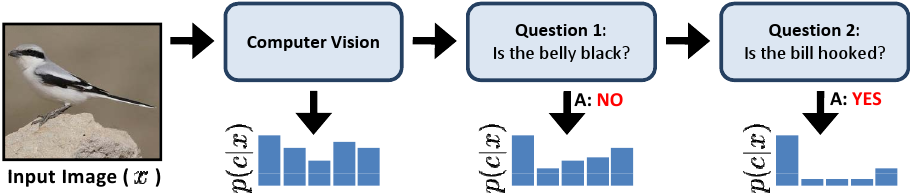
\includegraphics[width=\textwidth]{hitl_intro_2}
		\caption{نحوه به روزرسانی تخمین با پرسش از کاربر}
		\label{fig:fg_class:hil:up}
	\end{subfigure}
	\begin{subfigure}[h]{0.6\textwidth}
		\centering
		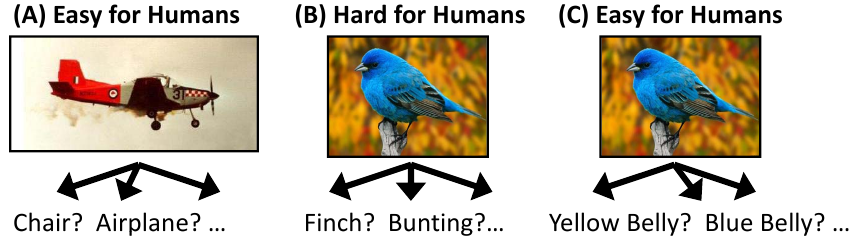
\includegraphics[width=\textwidth]{hitl_intro_1}
		\caption{انسان به چه سؤالاتی می‌تواند پاسخ دهد؟}
		\label{fig:fg_class:hil:int}
	\end{subfigure}
	\caption{نمای کلی روش همراه با انسان}
	\label{fig:fg_class:hil}
\end{figure}

در این روش هدف این است که دسته‌بندی نه به صورت کاملاً خودکار بلکه با کمک انسان و به صورت نیمه خودکار صورت بگیرد. سامانه بدین صورت کار می‌کند که پس از دریافت تصویر ورودی، سامانه از کاربر تعدادی سؤال می‌پرسد (برای مثال آیا رنگ بال پرنده آبی است یا خیر؟) پس از پاسخ به این سؤال سامانه تخمین خود از دسته‌ای که تصویر مربوط به آن است را به روز می‌کند (شکل
\ref{fig:fg_class:hil:up}).
این ایده از آنجا آمده است که دسته‌بندی معمولی برای انسان کار راحتی است ولی دسته‌بندی ریزدانه‌ای کار سختی است و افراد غیر متخصص توانایی انجام دقیق آن را ندارند. ولی تشخیص صفت‌های یک دسته‌ی ریزدانه‌ای مثل رنگ یک جزء کار آسانی برای انسان است (شکل
\ref{fig:fg_class:hil:int}). 
در
\cite{branson2010}
سامانه به گونه‌ای طراحی شده است که با کمترین تعداد پرسش بهترین نتیجه دسته‌بندی حاصل شود.

فرض کنید که دسته‌های ما
$c \in \{1, ..., C\}$ باشند.
در هر گام هدف استفاده از اطلاعات درون تصویر و سابقه‌ی پرسش‌ها و پاسخ‌های انجام شده تا به حال برای انتخاب سؤال بعدی است.
فرض کنید که
$Q = \{q_1, ..., q_n\}$
 مجموعه کل پرسش‌ها باشد،
$A_i$ پاسخ‌های ممکن به سؤال
$q_i$ است.
$a_i \in A_i$
متغییر تصادفی پاسخ کاربر به سؤال است. کاربر به غیر از پاسخ می‌توان اطمینان خود را از پاسخی که داده است را هم مشخص کند، که با
$r_i$ نمایش داده می‌شود و
$r_i \in \mathcal{V}$. برای مثال می‌توانیم قرار دهیم
$\mathcal{V} = \{ \text{حدس, تقریبا, مطمئن} \}$
پس کاربر زوج مرتب متغییر‌های تصادفی
$u_i = ( a_i, r_i )$
را به سامانه خواهد داد.
در هر زمان $t$ باید سؤال
$q_{j(t)}$ را انتخاب کرد
$j(t) \in \{ 1, ..., n \} $.
تعریف می‌کنیم
$ U^{t-1} = \{ u_{j(1)}, ..., u_{j(t-1)} \} $
مجموعه‌ی پاسخ‌هایی است که در گام‌های قبلی توسط کاربر پاسخ داده شده است.
همچنین
$I(c; u_i | x, U^{t-1})$ را امید ریاضی بهره اطلاعات در صورت بیان کردن سؤال
$q_i$ تعریف می‌کنیم.
حال سؤالی را انتخاب می‌کنیم که امید ریاضی ما از بهره اطلاعات را بیشینه کند. امید ریاضی بهره اطالعات پس از ساده‌ سازی به صورت زیر خواهد بود:
\begin{equation}
	\label{equ:fg_class:hil}
	I(c; u_i | x, U^{t-1}) = \sum_{u_i \in A_i \times \mathcal{V}} p(u_i | x, U ^{t-1}) \bigg( H(c| x, u_i \cup U ^{t-1}) - H( c | x, U ^{t-1} ) \bigg)
\end{equation}
و همچنین داریم:
\begin{equation}
	\label{equ:fg_class:hil_2}
	H( c | x, U ^{t-1} ) = - \sum_{c=1}^{C} p(c|x, U ^{t-1}) log p(c|x, U ^{t-1})
\end{equation}
در معادله‌ی
\ref{equ:fg_class:hil}
احتمال
$p(u_i | x, U ^{t-1})$
را مدل کاربر و در معادله‌ی
\ref{equ:fg_class:hil_2}
احتمال
$p(c|x, U ^{t-1})$
مدل بینایی ماشین تعریف می‌کنیم. که بستگی به مدلی که انتخاب می‌کنیم می‌تواند متفاوت باشد.

نتایج بدست آمده در این
\cite{branson2010}
مقاله نیز جالب است.
اگر هیچ سؤالی پرسیده نشود، دقت دسته‌بندی ۱۹ درصد است و با بیست سؤال دقت به بالای ۵۰ درصد ارتقا پیدا می‌کند.

این روش از نظر تئوری بسیار زیباست ولی هدف ما دسته‌بندی کاملا خودکار است، به همین خاطر از این روش‌ها می‌گذریم.

\subsection{روش‌های جدید دیگر}\label{sec:fg_class:new}
در سال‌های اخیر روش‌های مختلفی برای حل مسئله دسته‌بندی ریزدانه‌ای تصاویر مطرح شده است که دسته‌بندی آن‌ها سخت است. در ادامه به چند محور مشترک در این روش‌ها خواهیم پرداخت.
\subsubsection{پیدا کردن اجزای مهم به صورت خودکار}
\begin{figure}[t]
	\centering
	\begin{subfigure}[h]{0.35\textwidth}
		\centering
		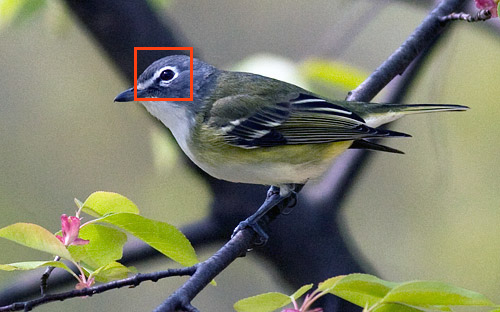
\includegraphics[height=3 cm]{vireo_1}
		\caption{\lr{Blue headed vireo}}
	\end{subfigure}
	\begin{subfigure}[h]{0.35\textwidth}
		\centering
		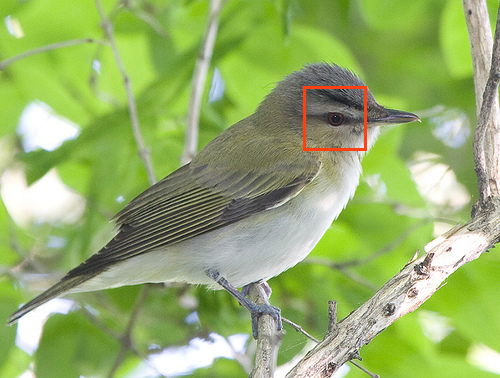
\includegraphics[height=3 cm]{vireo_2}
		\caption{\lr{Red eyed vireo}}
	\end{subfigure}
	\caption{دوگونه‌ی پرنده که در رنگ اطراف چشم تفاوت دارند}
	\label{fig:fg_class:part_diff}
\end{figure}
بسیاری از روش‌ها
\cite{yao2011, yao2012, style_aware, poof}
سعی می‌کنند به صورت خودکار بخش‌هایی از تصویر را پیدا کنند که قابلیت تمایز بالایی دارند. برای درک بهتر به تصویر دو گونه‌ی پرنده شکل
\ref{fig:fg_class:part_diff}
نگاه کنید. پیدا کردن تفاوت بین این دو گونه تنها در صورتی که بتوانیم چشم‌های پرنده را در تصویر پیدا کنیم امکان پذیر است. این روش‌ها اکثراً بر پایه‌ی محاسبات سنگینی هستند که در گام‌های پیاپی سامانه‌های تشخیص شیء
\footnote{\lr{Object detection}} مخصوص پیدا کردن این اجزاء تمایز دهنده را آموزش می‌دهند که کار بسیار سنگینی از نظر محاسباتی است.
(ما توانایی محاسباتی آن را نداریم.)

بهترین نتیجه‌ای که این روش‌ها می‌گیرند
\cite{poof}
بر روی پایگاه داده‌ی
\cite{cub2002011}
برابر ۵۶.۸ درصد است.
نکته جالب این است که اگر از اجزای داده شده اصلی استفاده کنند دقت این روش به ۷۳.۳ درصد افزایش می‌یابد که اهمیت مکان اعضا را نشان می‌دهد.
دیگر کارهای در این ارتباط پیدا کردن اجزا توسط جمع سپاری
\footnote{\lr{Crowdsourcing}}
است
\cite{deng2013}
که به خاطر خودکار نبودن مورد بررسی قرار نمی‌گیرد.

\subsubsection{انتقال اطلاعات از داده‌های آموزشی به داده‌های آزمایشی}
اهمیت مکان اجزا در قسمت قبل بیان شد. حال سؤال این است که اگر اطلاعات اجزا را در داده‌های آموزشی داشته باشیم، آیا می‌توانیم در داده‌های آزمایشی این اطلاعات را بدست آوریم. واضح است که هرچه در زمان آزمایش نیاز به اطلاعات کمتری داشته باشیم بهتر است. مقالات جدید
\cite{gavves2013, goring2014}
بر اساس مقاله مهم
\cite{esvm}
سعی بر این کار دارند و نتایج بسیار خوبی نیز کسب می‌کنند. فرض این روش‌ها این است که در صورتی که برای داده‌ی آزمایشی، از بین داده‌های آموزشی موردی را پیدا کنیم که از نظر شکل
\footnote{\lr{Shape}}
به داده‌ی آزمایشی شبیه باشند، می‌توان اطلاعات اجزا را از آن داده‌های آموزشی به داده‌ی آزمایشی انتقال داد و تخمینی از مکان اجزا بدست آورد. با این تخمین ویژگی‌های هسته‌ی فیشر یا کیسه‌ای از لغات را برای هر کدام از اجزا بدست می‌آورد، سپس دسته‌بندی را با این ویژگی‌ها انجام می‌دهد. با این ایده روش
\cite{gavves2013}
به دقت میانگین ۶۲.۷ درصد و روش
\cite{goring2014}
به دقت میانگین ۵۷.۸۴ درصد دست می‌یابد.

\subsubsection{یادگیری عمیق}

همانطور که در بخش
\ref{sec:img_class:dl}
گفته شد، روش‌های یادگیری عمیق به خاطر قابلیت‌های بالایشان در یادگیری ویژگی سریعاً برای دسته‌بندی ریزدانه‌ای نیز مورد استفاده قرار گرفتند. برای نمونه در این رابطه می‌توان به
\cite{razavian2014, krause2014, partrcnn}
اشاره کرد. این روش‌ها به قدری قوی هستند که اگر حتی ویژگی‌ها بر روی پایگاه داده‌ی دیگری به جز آنچه بر روی آن آزمایش انجام می دهیم نیز آموزش داده شوند، باز نتایج بسیار خوبی کسب می‌کنند
\cite{razavian2014}.
به علت قدرت این روش‌ها ما بر روی آن‌ها آزمایشاتی انجام دادیم که در بخش
\ref{sec:results}
به آن اشاره می‌کنیم. همچنین دقت روش‌های مختلف در بخش
\ref{sec:results}
با یکدیگر مقایسه شده‌اند.
%%%%%%%%%%%%%%%%%%%%%%%%%%%%%%%%%%%%%%%%%%%%%%%%%%%%%%%%%%%%%%%%%
\section{روش‌پیشنهادی و جمع‌بندی}\label{sec:conc}
آنچه بیان شد، خلاصه‌ای از روش‌های مهم در دسته‌بندی تصویر معمولی و دسته‌بندی ریزدانه‌ای تصویر بود. دیدیم که در روش‌هایی که بر پایه‌ی کیسه‌ای از لغات هستند با کدینگ هسته‌ی فیشر بهترین نتیجه را کسب می‌کنند. از این روش‌ها بهتر روش‌های مبتنی بر یادگیری عمیق بودند که مطالعه تئوری آن‌ها فراتر از مباحث این گزارش می‌باشد. لذا در ادامه به این روش‌ها به عنوان یک روش استخراج ویژگی نگاه می‌کنیم و به جزئیات آن‌ها نمی‌پردازیم. در ادامه به بررسی روش پیشنهادی می‌پردازیم.
\subsection{روش پیشنهادی و نتایج اولیه}\label{sec:results}
مطابق بهترین روش‌ها پیشنهاد می‌شود که برای استخراج ویژگی از ویژگی‌ها مدل‌های یادگیری عمیق استفاده شود. همانطور که در
\cite{razavian2014}
نیز اشاره شده است، لازم نیست که شبکه عصبی مصنوعی عمیق را برای هر پایگاه‌داده‌ای آموزش دهیم (البته در برخی موارد آموزش شبکه عصبی مصنوعی عمیق با توجه به تعداد کم داده‌های ممکن نیست)، اگر یک بار شبکه بر روی پایگاه‌داده‌ای مثل
\lr{ILSVRC} \cite{ilsvrc}
آموزش داده شود می‌توان از همان ویژگی‌های یادگرفته شده برای پایگاه داده‌های دیگر نیز استفاده کرد
\cite{razavian2014}.
\begin{figure}[t]
	\centering
	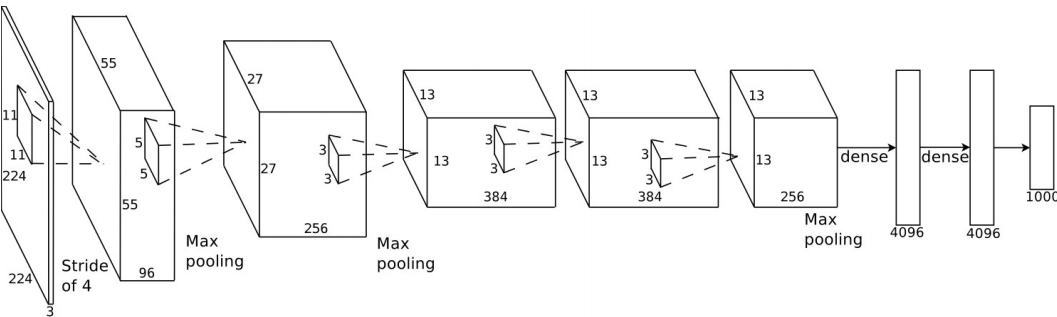
\includegraphics[height= 2.5 cm]{alexnet}
	\caption{ساختار شبکه عصبی موسوم به
	\lr{AlexNet}\cite{alexnet} که در آزمایشات مورد استفاده قرار گرفته است.}
	\label{fig:conc:alexnet}
\end{figure}
برای پیاده‌سازی ما از ابزار متن باز
\lr{Caffe} \cite{caffe}
استفاده کردیم. به عنوان مدل هم از شبکه عصبی معروف
\lr{AlexNet} \cite{alexnet}
که در شکل
\ref{fig:conc:alexnet} قابل مشاهده است، استفاده شده.
این شبکه ابتدا با داده‌های
\lr{ILSVRC} \cite{ilsvrc}
آموزش داده شده است و برای استخراج ویژگی توسط راه حل پیشنهادی ما مورد استفاده قرار می‌گیرید. به عنوان مدل یادگیرنده از
\lr{SVM} \cite{svm}
با هسته‌ی خطی و مقدار
$C = 3$
استفاده شد. با این ابزارها سه آزمایش مختلف انجام گرفت. که تفاوت آن‌ها در داده‌های آموزشی است. پایگاه داده مورد استفاده نیز
\lr{CUB-200-2011} \cite{cub2002011}
انتخاب شد که به راحتی بتوان با روش‌های مختلف مقایسه انجام داد.

\textbf{آزمایش اول}:
در آزمایش اول از هیچ اطلاعات کمکی مثل جعبه دور شی‌ء و اجزا استفاده نشد. عکس‌های آموزشی و آزمایشی برای استخراج ویژگی بعد از تغییر اندازه به
$256 \times 256$
به شبکه عصبی به عنوان ورودی داده می‌شد و اطلاعات لایه‌ی یکی مانده به آخر به عنوان ویژگی استخراج می‌شد. این بردار ویژگی دارای ۴۰۹۶ بعد بود. سپس با این ویژگی‌ها یک
\lr{SVM} خطی آموزش داده می‌شد.
داده‌های آموزش و آزمایش نیز طبق تقسیم‌بندی پایگاه داده استفاده شد. دقت در این روش برابر ۴۵.۴۴ درصد است.

\textbf{آزمایش دوم}:
فرق آزمایش اول با آزمایش دوم در این بود که ابتدا با استفاده از جعبه دور شیء، تصویر بریده می‌شود، سپس همان مراحل آزمایش اول تکرار می‌شود. دقت در این آزمایش به میزان قابل توجهی افزایش پیدا کرد و به ۵۵.۶۲ درصد رسید. این موضوع نشان دهنده‌ی گمراه کننده بودن اطلاعات موجود در پس زمینه‌ی اشیاء در این پایگاه داده است. پس هرچه بتوان این اطلاعات را حذف کرد موفقیت بیشتری حاصل می‌شود.

\textbf{آزمایش سوم}:
در این آزمایش ویژگی‌های استخراج شده در آزمایش اول و دوم به هم چسبانده شد و یک بردار ویژگی ۸۱۹۲ بعدی برای هر تصویر بدست آمد. با این کار نتایج باز هم افزایش یافت و به ۵۷.۸۳ درصد رسید که قابل قبول است.

\textbf{مقایسه با روش‌های مهم}:
در جدول زیر آزمایش‌های خود را با بهترین نتایج مقایسه‌ می‌کنیم.

\begin{table}
\centering
\caption{مقایسه میانگین دقت روش ارائه شده با روش‌های دیگر}
\label{tbl:result}
\footnotesize{
\begin{tabular}{|c|c|c|c|c|}
\hline روش & سال ارائه & استفاده از جعبه دور & استفاده از اطلاعات اجزا & دقت ٪\\ 
\hline
\hline  	CUB \cite{cub2002011} 	& 2011 & \cmark & 		& 10.3\\
		CUB \cite{cub2002011} 	& 2011 & \cmark & \cmark	& 17.3\\
		PPK \cite{ppk}			& 2012 & \cmark &		& 28.18\\
		style \cite{style_aware}	& 2013 & \cmark &		& 41.01\\
		POOF \cite{poof}		& 2013 & \cmark &		& 56.8 \\
		Alignments \cite{gavves2013}& 2013 & \cmark &		& \textbf{62.7} \\
		DPD \cite{dpd}			& 2013 & \cmark & \cmark	& 51.0 \\
		Decafe \cite{decaf}		& 2014 & \cmark & 		& \textbf{65.0} \\
		PNDCN \cite{partrcnn}	& 2014 & \cmark &		& \textbf{75.7} \\
		CNN \cite{razavian2014}	& 2014 & \cmark &		& 53.3 \\
		CNN-aug \cite{razavian2014} & 2014 & \cmark &		& \textbf{61.08} \\
\hline 	Ours-1				& - 	   &		&		& 45.44 \\
		Ours-2				& -       & \cmark &		& 55.62 \\
		Ours-3				& -       & \cmark &		& \textbf{57.83} \\
\hline 
\end{tabular} 
}
\end{table}
\subsection{کارهای آینده}\label{sec:future}
همانطور که در جدول
\ref{tbl:result}
می‌توان دید روش پیشنهادی نتایج قابل مقایسه و خوبی نسبت به روش‌های دیگر دارد. البته فعلاً روش ما از اطلاعات سه‌بعدی، اطلاعات اجزا در داده‌های آموزشی و از افزودن داده‌های آموزشی
\footnote{\lr{Data augmentation}}
استفاده نمی‌کند. همچنین روش‌ها معمولاً بر روی تمام دسته‌ها خوب جواب نمی‌دهد و اینکه روش‌های مختلف بر روی دسته‌های مختلفی خوب عمل می‌کنند، تحلیل دلیل ضعف و قوت هر کدام از روش‌ها می‌تواند به ما در طراحی مدل‌های بهتر کمک کند.

\begin{table}[h]
\centering
\caption{زمان‌بندی انجام پروژه}
\label{tbl:schedule1}
\footnotesize{
\begin{tabular}{|c|c|c|c|}
\hline عنوان فعالیت & مدت زمان لازم & درصد پیشرفت & زمان اتمام \\ 
\hline \hline مطالعه روش‌های پیشین برای دسته‌بندی معمولی و دسته‌بندی ریزدانه‌ای & ۰.۵ ماه & ۱۰۰ & شهریور ۹۳ \\ 
\hline پیاده‌سازی و اجرای روش‌های پایه & ۱ ماه & ۵۰ & آبان ۹۳ \\ 
\hline پیاده‌سازی روش پیشنهادی جدید & ۳ ماه & ۲۰ & بهمن ۹۳ \\ 
\hline نگارش پایان‌نامه & ۱ ماه & ۱۰ & بهمن ۹۳ \\ 
\hline جمع‌بندی نتایج و نوشتن مقاله & ۰.۵ ماه & ۰ & اسفند ۹۳ \\ 
\hline 
\end{tabular} 
}
\end{table}

%%%%%%%%%%%%%%%%%%%%%%%%%%%%%%%%%%%%%%%%%%%%%%%%%%%%%%%%%%%%%%%%%
\linespread{1}
\small
\setlength{\parskip}{0pt}
\setlength{\parsep}{0pt}

\renewcommand{\bibname}{مراجع}
\begin{latin}
\bibliographystyle{IEEEtran}
%\bibliography{IEEEfull,ref}
\bibliography{IEEEabrv,ref}
\end{latin}



\section*{واژه‌نامه}
%\begin{LTR}
\begin{multicols}{3}
\theendnotes 
\end{multicols}
%\end{LTR}
\end{document}
